\documentclass[twoside]{book}

% Packages required by doxygen
\usepackage{fixltx2e}
\usepackage{calc}
\usepackage{doxygen}
\usepackage[export]{adjustbox} % also loads graphicx
\usepackage{graphicx}
\usepackage[utf8]{inputenc}
\usepackage{makeidx}
\usepackage{multicol}
\usepackage{multirow}
\PassOptionsToPackage{warn}{textcomp}
\usepackage{textcomp}
\usepackage[nointegrals]{wasysym}
\usepackage[table]{xcolor}

% Font selection
\usepackage[T1]{fontenc}
\usepackage[scaled=.90]{helvet}
\usepackage{courier}
\usepackage{amssymb}
\usepackage{sectsty}
\renewcommand{\familydefault}{\sfdefault}
\allsectionsfont{%
  \fontseries{bc}\selectfont%
  \color{darkgray}%
}
\renewcommand{\DoxyLabelFont}{%
  \fontseries{bc}\selectfont%
  \color{darkgray}%
}
\newcommand{\+}{\discretionary{\mbox{\scriptsize$\hookleftarrow$}}{}{}}

% Page & text layout
\usepackage{geometry}
\geometry{%
  a4paper,%
  top=2.5cm,%
  bottom=2.5cm,%
  left=2.5cm,%
  right=2.5cm%
}
\tolerance=750
\hfuzz=15pt
\hbadness=750
\setlength{\emergencystretch}{15pt}
\setlength{\parindent}{0cm}
\setlength{\parskip}{3ex plus 2ex minus 2ex}
\makeatletter
\renewcommand{\paragraph}{%
  \@startsection{paragraph}{4}{0ex}{-1.0ex}{1.0ex}{%
    \normalfont\normalsize\bfseries\SS@parafont%
  }%
}
\renewcommand{\subparagraph}{%
  \@startsection{subparagraph}{5}{0ex}{-1.0ex}{1.0ex}{%
    \normalfont\normalsize\bfseries\SS@subparafont%
  }%
}
\makeatother

% Headers & footers
\usepackage{fancyhdr}
\pagestyle{fancyplain}
\fancyhead[LE]{\fancyplain{}{\bfseries\thepage}}
\fancyhead[CE]{\fancyplain{}{}}
\fancyhead[RE]{\fancyplain{}{\bfseries\leftmark}}
\fancyhead[LO]{\fancyplain{}{\bfseries\rightmark}}
\fancyhead[CO]{\fancyplain{}{}}
\fancyhead[RO]{\fancyplain{}{\bfseries\thepage}}
\fancyfoot[LE]{\fancyplain{}{}}
\fancyfoot[CE]{\fancyplain{}{}}
\fancyfoot[RE]{\fancyplain{}{\bfseries\scriptsize Generated by Doxygen }}
\fancyfoot[LO]{\fancyplain{}{\bfseries\scriptsize Generated by Doxygen }}
\fancyfoot[CO]{\fancyplain{}{}}
\fancyfoot[RO]{\fancyplain{}{}}
\renewcommand{\footrulewidth}{0.4pt}
\renewcommand{\chaptermark}[1]{%
  \markboth{#1}{}%
}
\renewcommand{\sectionmark}[1]{%
  \markright{\thesection\ #1}%
}

% Indices & bibliography
\usepackage{natbib}
\usepackage[titles]{tocloft}
\setcounter{tocdepth}{3}
\setcounter{secnumdepth}{5}
\makeindex

% Hyperlinks (required, but should be loaded last)
\usepackage{ifpdf}
\ifpdf
  \usepackage[pdftex,pagebackref=true]{hyperref}
\else
  \usepackage[ps2pdf,pagebackref=true]{hyperref}
\fi
\hypersetup{%
  colorlinks=true,%
  linkcolor=blue,%
  citecolor=blue,%
  unicode%
}

% Custom commands
\newcommand{\clearemptydoublepage}{%
  \newpage{\pagestyle{empty}\cleardoublepage}%
}

\usepackage{caption}
\captionsetup{labelsep=space,justification=centering,font={bf},singlelinecheck=off,skip=4pt,position=top}

%===== C O N T E N T S =====

\begin{document}

% Titlepage & ToC
\hypersetup{pageanchor=false,
             bookmarksnumbered=true,
             pdfencoding=unicode
            }
\pagenumbering{alph}
\begin{titlepage}
\vspace*{7cm}
\begin{center}%
{\Large Pràctica P\+R\+O2 primavera 2020. Pau Antonio Soler \\[1ex]\large versió 1 21-\/abr-\/2020 }\\
\vspace*{1cm}
{\large Generated by Doxygen 1.8.13}\\
\end{center}
\end{titlepage}
\clearemptydoublepage
\pagenumbering{roman}
\tableofcontents
\clearemptydoublepage
\pagenumbering{arabic}
\hypersetup{pageanchor=true}

%--- Begin generated contents ---
\chapter{Pràctica P\+R\+O2\+: Construcció d\textquotesingle{}un arbre filogenètic.}
\label{index}\hypertarget{index}{}Construcció de l\textquotesingle{}arbre filogenètic per a un conjunt d\textquotesingle{}N espècies utilitzant el mètode de W\+P\+G\+MA. 
\chapter{Class Index}
\section{Class List}
Here are the classes, structs, unions and interfaces with brief descriptions\+:\begin{DoxyCompactList}
\item\contentsline{section}{\hyperlink{class_bin_tree}{Bin\+Tree$<$ T $>$} }{\pageref{class_bin_tree}}{}
\item\contentsline{section}{\hyperlink{class_cjt__clusters}{Cjt\+\_\+clusters} \\*Representa un conjunt de clústers }{\pageref{class_cjt__clusters}}{}
\item\contentsline{section}{\hyperlink{class_cjt__especies}{Cjt\+\_\+especies} \\*Representa un conjunt d\textquotesingle{}espècies }{\pageref{class_cjt__especies}}{}
\item\contentsline{section}{\hyperlink{class_cluster}{Cluster} \\*Representa un clúster }{\pageref{class_cluster}}{}
\item\contentsline{section}{\hyperlink{class_especie}{Especie} \\*Representa una entitat o espècie amb atributs identificador i gen }{\pageref{class_especie}}{}
\end{DoxyCompactList}

\chapter{File Index}
\section{File List}
Here is a list of all files with brief descriptions\+:\begin{DoxyCompactList}
\item\contentsline{section}{\hyperlink{_bin_tree_8hh}{Bin\+Tree.\+hh} }{\pageref{_bin_tree_8hh}}{}
\item\contentsline{section}{\hyperlink{_cjt__clusters_8hh}{Cjt\+\_\+clusters.\+hh} \\*Especificació de la classe \hyperlink{class_cjt__clusters}{Cjt\+\_\+clusters} }{\pageref{_cjt__clusters_8hh}}{}
\item\contentsline{section}{\hyperlink{_cjt__especies_8hh}{Cjt\+\_\+especies.\+hh} \\*Especificació de la classe \hyperlink{class_cjt__especies}{Cjt\+\_\+especies} }{\pageref{_cjt__especies_8hh}}{}
\item\contentsline{section}{\hyperlink{_cluster_8hh}{Cluster.\+hh} \\*Especificació de la classe \hyperlink{class_cluster}{Cluster} }{\pageref{_cluster_8hh}}{}
\item\contentsline{section}{\hyperlink{_especie_8hh}{Especie.\+hh} \\*Especificació de la classe \hyperlink{class_especie}{Especie} }{\pageref{_especie_8hh}}{}
\item\contentsline{section}{\hyperlink{main_8cc}{main.\+cc} \\*Programa principal de la {\itshape Construcció d\textquotesingle{}un arbre filogenètic} }{\pageref{main_8cc}}{}
\end{DoxyCompactList}

\chapter{Class Documentation}
\hypertarget{class_bin_tree}{}\section{Bin\+Tree$<$ T $>$ Class Template Reference}
\label{class_bin_tree}\index{Bin\+Tree$<$ T $>$@{Bin\+Tree$<$ T $>$}}
\subsection*{Public Member Functions}
\begin{DoxyCompactItemize}
\item 
\hyperlink{class_bin_tree_a47eef22d29cd023449d97c073c08e5b6}{Bin\+Tree} ()
\item 
\hyperlink{class_bin_tree_a1ab686e0bcf990093ff91fe71744c1a4}{Bin\+Tree} (const T \&x)
\item 
\hyperlink{class_bin_tree_adb7eeff76d08130c943b36af215eb521}{Bin\+Tree} (const T \&x, const \hyperlink{class_bin_tree}{Bin\+Tree} \&\hyperlink{class_bin_tree_a82108db4c1b08d1f111027788c196d4e}{left}, const \hyperlink{class_bin_tree}{Bin\+Tree} \&\hyperlink{class_bin_tree_aff8e96651b27284c329667b5ad3e4d0b}{right})
\item 
bool \hyperlink{class_bin_tree_a74cda259ba5c25b8ee38ed4dc33e4fad}{empty} () const
\item 
\hyperlink{class_bin_tree}{Bin\+Tree} \hyperlink{class_bin_tree_a82108db4c1b08d1f111027788c196d4e}{left} () const
\item 
\hyperlink{class_bin_tree}{Bin\+Tree} \hyperlink{class_bin_tree_aff8e96651b27284c329667b5ad3e4d0b}{right} () const
\item 
const T \& \hyperlink{class_bin_tree_a734e785b089c87b49187ee7c58edf5f3}{value} () const
\end{DoxyCompactItemize}


\subsection{Detailed Description}
\subsubsection*{template$<$typename T$>$\newline
class Bin\+Tree$<$ T $>$}



Definition at line 15 of file Bin\+Tree.\+hh.



\subsection{Constructor \& Destructor Documentation}
\mbox{\Hypertarget{class_bin_tree_a47eef22d29cd023449d97c073c08e5b6}\label{class_bin_tree_a47eef22d29cd023449d97c073c08e5b6}} 
\index{Bin\+Tree@{Bin\+Tree}!Bin\+Tree@{Bin\+Tree}}
\index{Bin\+Tree@{Bin\+Tree}!Bin\+Tree@{Bin\+Tree}}
\subsubsection{\texorpdfstring{Bin\+Tree()}{BinTree()}\hspace{0.1cm}{\footnotesize\ttfamily [1/3]}}
{\footnotesize\ttfamily template$<$typename T$>$ \\
\hyperlink{class_bin_tree}{Bin\+Tree}$<$ T $>$\+::\hyperlink{class_bin_tree}{Bin\+Tree} (\begin{DoxyParamCaption}{ }\end{DoxyParamCaption})}



Definition at line 44 of file Bin\+Tree.\+hh.


\begin{DoxyCode}
45     :   p(\textcolor{keyword}{nullptr})
46     \{   \}
\end{DoxyCode}
\mbox{\Hypertarget{class_bin_tree_a1ab686e0bcf990093ff91fe71744c1a4}\label{class_bin_tree_a1ab686e0bcf990093ff91fe71744c1a4}} 
\index{Bin\+Tree@{Bin\+Tree}!Bin\+Tree@{Bin\+Tree}}
\index{Bin\+Tree@{Bin\+Tree}!Bin\+Tree@{Bin\+Tree}}
\subsubsection{\texorpdfstring{Bin\+Tree()}{BinTree()}\hspace{0.1cm}{\footnotesize\ttfamily [2/3]}}
{\footnotesize\ttfamily template$<$typename T$>$ \\
\hyperlink{class_bin_tree}{Bin\+Tree}$<$ T $>$\+::\hyperlink{class_bin_tree}{Bin\+Tree} (\begin{DoxyParamCaption}\item[{const T \&}]{x }\end{DoxyParamCaption})\hspace{0.3cm}{\ttfamily [explicit]}}



Definition at line 49 of file Bin\+Tree.\+hh.


\begin{DoxyCode}
49                                   \{
50         p = make\_shared<Node>(x, \textcolor{keyword}{nullptr}, \textcolor{keyword}{nullptr});
51     \}
\end{DoxyCode}
\mbox{\Hypertarget{class_bin_tree_adb7eeff76d08130c943b36af215eb521}\label{class_bin_tree_adb7eeff76d08130c943b36af215eb521}} 
\index{Bin\+Tree@{Bin\+Tree}!Bin\+Tree@{Bin\+Tree}}
\index{Bin\+Tree@{Bin\+Tree}!Bin\+Tree@{Bin\+Tree}}
\subsubsection{\texorpdfstring{Bin\+Tree()}{BinTree()}\hspace{0.1cm}{\footnotesize\ttfamily [3/3]}}
{\footnotesize\ttfamily template$<$typename T$>$ \\
\hyperlink{class_bin_tree}{Bin\+Tree}$<$ T $>$\+::\hyperlink{class_bin_tree}{Bin\+Tree} (\begin{DoxyParamCaption}\item[{const T \&}]{x,  }\item[{const \hyperlink{class_bin_tree}{Bin\+Tree}$<$ T $>$ \&}]{left,  }\item[{const \hyperlink{class_bin_tree}{Bin\+Tree}$<$ T $>$ \&}]{right }\end{DoxyParamCaption})\hspace{0.3cm}{\ttfamily [explicit]}}



Definition at line 54 of file Bin\+Tree.\+hh.


\begin{DoxyCode}
54                                                                              \{
55         p = make\_shared<Node>(x, left.p, right.p);
56     \}
\end{DoxyCode}


\subsection{Member Function Documentation}
\mbox{\Hypertarget{class_bin_tree_a74cda259ba5c25b8ee38ed4dc33e4fad}\label{class_bin_tree_a74cda259ba5c25b8ee38ed4dc33e4fad}} 
\index{Bin\+Tree@{Bin\+Tree}!empty@{empty}}
\index{empty@{empty}!Bin\+Tree@{Bin\+Tree}}
\subsubsection{\texorpdfstring{empty()}{empty()}}
{\footnotesize\ttfamily template$<$typename T$>$ \\
bool \hyperlink{class_bin_tree}{Bin\+Tree}$<$ T $>$\+::empty (\begin{DoxyParamCaption}{ }\end{DoxyParamCaption}) const}



Definition at line 59 of file Bin\+Tree.\+hh.


\begin{DoxyCode}
59                         \{
60         \textcolor{keywordflow}{return} not p;
61     \}
\end{DoxyCode}
\mbox{\Hypertarget{class_bin_tree_a82108db4c1b08d1f111027788c196d4e}\label{class_bin_tree_a82108db4c1b08d1f111027788c196d4e}} 
\index{Bin\+Tree@{Bin\+Tree}!left@{left}}
\index{left@{left}!Bin\+Tree@{Bin\+Tree}}
\subsubsection{\texorpdfstring{left()}{left()}}
{\footnotesize\ttfamily template$<$typename T$>$ \\
\hyperlink{class_bin_tree}{Bin\+Tree} \hyperlink{class_bin_tree}{Bin\+Tree}$<$ T $>$\+::left (\begin{DoxyParamCaption}{ }\end{DoxyParamCaption}) const}



Definition at line 64 of file Bin\+Tree.\+hh.


\begin{DoxyCode}
64                           \{
65         assert(not \hyperlink{class_bin_tree_a74cda259ba5c25b8ee38ed4dc33e4fad}{empty}());
66         \textcolor{keywordflow}{return} \hyperlink{class_bin_tree_a47eef22d29cd023449d97c073c08e5b6}{BinTree}(p->left);
67     \}
\end{DoxyCode}
\mbox{\Hypertarget{class_bin_tree_aff8e96651b27284c329667b5ad3e4d0b}\label{class_bin_tree_aff8e96651b27284c329667b5ad3e4d0b}} 
\index{Bin\+Tree@{Bin\+Tree}!right@{right}}
\index{right@{right}!Bin\+Tree@{Bin\+Tree}}
\subsubsection{\texorpdfstring{right()}{right()}}
{\footnotesize\ttfamily template$<$typename T$>$ \\
\hyperlink{class_bin_tree}{Bin\+Tree} \hyperlink{class_bin_tree}{Bin\+Tree}$<$ T $>$\+::right (\begin{DoxyParamCaption}{ }\end{DoxyParamCaption}) const}



Definition at line 70 of file Bin\+Tree.\+hh.


\begin{DoxyCode}
70                            \{
71         assert(not \hyperlink{class_bin_tree_a74cda259ba5c25b8ee38ed4dc33e4fad}{empty}());
72         \textcolor{keywordflow}{return} \hyperlink{class_bin_tree_a47eef22d29cd023449d97c073c08e5b6}{BinTree}(p->right);
73     \}
\end{DoxyCode}
\mbox{\Hypertarget{class_bin_tree_a734e785b089c87b49187ee7c58edf5f3}\label{class_bin_tree_a734e785b089c87b49187ee7c58edf5f3}} 
\index{Bin\+Tree@{Bin\+Tree}!value@{value}}
\index{value@{value}!Bin\+Tree@{Bin\+Tree}}
\subsubsection{\texorpdfstring{value()}{value()}}
{\footnotesize\ttfamily template$<$typename T$>$ \\
const T\& \hyperlink{class_bin_tree}{Bin\+Tree}$<$ T $>$\+::value (\begin{DoxyParamCaption}{ }\end{DoxyParamCaption}) const}



Definition at line 76 of file Bin\+Tree.\+hh.


\begin{DoxyCode}
76                             \{
77         assert(not \hyperlink{class_bin_tree_a74cda259ba5c25b8ee38ed4dc33e4fad}{empty}());
78         \textcolor{keywordflow}{return} p->x;
79     \}
\end{DoxyCode}


The documentation for this class was generated from the following file\+:\begin{DoxyCompactItemize}
\item 
\hyperlink{_bin_tree_8hh}{Bin\+Tree.\+hh}\end{DoxyCompactItemize}

\hypertarget{class_cjt__clusters}{}\section{Cjt\+\_\+clusters Class Reference}
\label{class_cjt__clusters}\index{Cjt\+\_\+clusters@{Cjt\+\_\+clusters}}


Representa un conjunt de clústers.  


\subsection*{Public Member Functions}
\begin{DoxyCompactItemize}
\item 
\hyperlink{class_cjt__clusters_a10dd63eab0e8ea5b1ed13e81412d47a9}{Cjt\+\_\+clusters} ()
\begin{DoxyCompactList}\small\item\em Creadora per defecte. \end{DoxyCompactList}\item 
\hyperlink{class_cjt__clusters_aa52c1e5013ed206efccd70aaba9c037c}{Cjt\+\_\+clusters} (\hyperlink{class_cjt__especies}{Cjt\+\_\+especies} cesp)
\begin{DoxyCompactList}\small\item\em Creadora a partir d\textquotesingle{}un conjunt d\textquotesingle{}espècies. \end{DoxyCompactList}\item 
\hyperlink{class_cjt__clusters_aba7f00077ce77ba7963ac8084be4a000}{$\sim$\+Cjt\+\_\+clusters} ()
\begin{DoxyCompactList}\small\item\em Destructora per defecte. \end{DoxyCompactList}\item 
void \hyperlink{class_cjt__clusters_ae5d7fd65b9070ea2e7240d78fefd0f6e}{wpgma\+\_\+pas} ()
\begin{DoxyCompactList}\small\item\em Modificadora que aplica un pas de l\textquotesingle{}algorisme W\+P\+G\+MA. \end{DoxyCompactList}\item 
void \hyperlink{class_cjt__clusters_a755fca978c7d4b499e2c7b0963136354}{wpgma\+\_\+total} ()
\begin{DoxyCompactList}\small\item\em Modificadora que aplica l\textquotesingle{}algorisme W\+P\+G\+MA. \end{DoxyCompactList}\item 
void \hyperlink{class_cjt__clusters_ab243c775e0e2d64905ce744490d2f898}{taula\+\_\+distancies\+\_\+clusters} () const
\begin{DoxyCompactList}\small\item\em Consultora de taula de distàncies entre clústers. \end{DoxyCompactList}\item 
void \hyperlink{class_cjt__clusters_a0c0922c708fb014720a53bd560ebed61}{inicialitza\+\_\+cluster} (const \hyperlink{class_cjt__especies}{Cjt\+\_\+especies} \&cesp)
\begin{DoxyCompactList}\small\item\em Inicialitza el conjunt de clústers. \end{DoxyCompactList}\item 
void \hyperlink{class_cjt__clusters_ad023ea2a94f2629848f5c6b7162ac8d8}{escriure\+\_\+cluster} (const string \&id) const
\begin{DoxyCompactList}\small\item\em Operació d\textquotesingle{}escriptura de clúster. \end{DoxyCompactList}\item 
void \hyperlink{class_cjt__clusters_afdef4a4f7bd8ca2ecaf723c65cc10be0}{escriure\+\_\+arbre} () const
\begin{DoxyCompactList}\small\item\em Operació d\textquotesingle{}escriptura de l\textquotesingle{}arbre filogenètic. \end{DoxyCompactList}\end{DoxyCompactItemize}


\subsection{Detailed Description}
Representa un conjunt de clústers. 

Definition at line 17 of file Cjt\+\_\+clusters.\+hh.



\subsection{Constructor \& Destructor Documentation}
\mbox{\Hypertarget{class_cjt__clusters_a10dd63eab0e8ea5b1ed13e81412d47a9}\label{class_cjt__clusters_a10dd63eab0e8ea5b1ed13e81412d47a9}} 
\index{Cjt\+\_\+clusters@{Cjt\+\_\+clusters}!Cjt\+\_\+clusters@{Cjt\+\_\+clusters}}
\index{Cjt\+\_\+clusters@{Cjt\+\_\+clusters}!Cjt\+\_\+clusters@{Cjt\+\_\+clusters}}
\subsubsection{\texorpdfstring{Cjt\+\_\+clusters()}{Cjt\_clusters()}\hspace{0.1cm}{\footnotesize\ttfamily [1/2]}}
{\footnotesize\ttfamily Cjt\+\_\+clusters\+::\+Cjt\+\_\+clusters (\begin{DoxyParamCaption}{ }\end{DoxyParamCaption})}



Creadora per defecte. 

\begin{DoxyPrecond}{Precondition}
{\itshape cert} 
\end{DoxyPrecond}
\begin{DoxyPostcond}{Postcondition}
El resultat és un conjunt de clústers buit 
\end{DoxyPostcond}
\mbox{\Hypertarget{class_cjt__clusters_aa52c1e5013ed206efccd70aaba9c037c}\label{class_cjt__clusters_aa52c1e5013ed206efccd70aaba9c037c}} 
\index{Cjt\+\_\+clusters@{Cjt\+\_\+clusters}!Cjt\+\_\+clusters@{Cjt\+\_\+clusters}}
\index{Cjt\+\_\+clusters@{Cjt\+\_\+clusters}!Cjt\+\_\+clusters@{Cjt\+\_\+clusters}}
\subsubsection{\texorpdfstring{Cjt\+\_\+clusters()}{Cjt\_clusters()}\hspace{0.1cm}{\footnotesize\ttfamily [2/2]}}
{\footnotesize\ttfamily Cjt\+\_\+clusters\+::\+Cjt\+\_\+clusters (\begin{DoxyParamCaption}\item[{\hyperlink{class_cjt__especies}{Cjt\+\_\+especies}}]{cesp }\end{DoxyParamCaption})}



Creadora a partir d\textquotesingle{}un conjunt d\textquotesingle{}espècies. 

\begin{DoxyPrecond}{Precondition}
\char`\"{}cesp\char`\"{} és un conjunt d\textquotesingle{}espècies no buit 
\end{DoxyPrecond}
\begin{DoxyPostcond}{Postcondition}
El resultat és un conjunt de clústers format a partir de les espècies del conjunt d\textquotesingle{}espècies \char`\"{}cesp\char`\"{} 
\end{DoxyPostcond}
\mbox{\Hypertarget{class_cjt__clusters_aba7f00077ce77ba7963ac8084be4a000}\label{class_cjt__clusters_aba7f00077ce77ba7963ac8084be4a000}} 
\index{Cjt\+\_\+clusters@{Cjt\+\_\+clusters}!````~Cjt\+\_\+clusters@{$\sim$\+Cjt\+\_\+clusters}}
\index{````~Cjt\+\_\+clusters@{$\sim$\+Cjt\+\_\+clusters}!Cjt\+\_\+clusters@{Cjt\+\_\+clusters}}
\subsubsection{\texorpdfstring{$\sim$\+Cjt\+\_\+clusters()}{~Cjt\_clusters()}}
{\footnotesize\ttfamily Cjt\+\_\+clusters\+::$\sim$\+Cjt\+\_\+clusters (\begin{DoxyParamCaption}{ }\end{DoxyParamCaption})}



Destructora per defecte. 



\subsection{Member Function Documentation}
\mbox{\Hypertarget{class_cjt__clusters_ae5d7fd65b9070ea2e7240d78fefd0f6e}\label{class_cjt__clusters_ae5d7fd65b9070ea2e7240d78fefd0f6e}} 
\index{Cjt\+\_\+clusters@{Cjt\+\_\+clusters}!wpgma\+\_\+pas@{wpgma\+\_\+pas}}
\index{wpgma\+\_\+pas@{wpgma\+\_\+pas}!Cjt\+\_\+clusters@{Cjt\+\_\+clusters}}
\subsubsection{\texorpdfstring{wpgma\+\_\+pas()}{wpgma\_pas()}}
{\footnotesize\ttfamily void Cjt\+\_\+clusters\+::wpgma\+\_\+pas (\begin{DoxyParamCaption}{ }\end{DoxyParamCaption})}



Modificadora que aplica un pas de l\textquotesingle{}algorisme W\+P\+G\+MA. 

\begin{DoxyPrecond}{Precondition}
El paràmetre implícit està format per dos o més clústers 
\end{DoxyPrecond}
\begin{DoxyPostcond}{Postcondition}
El resultat és un conjunt de clústers modificat al aplicar un pas de l\textquotesingle{}algorisme W\+P\+G\+MA 
\end{DoxyPostcond}
\mbox{\Hypertarget{class_cjt__clusters_a755fca978c7d4b499e2c7b0963136354}\label{class_cjt__clusters_a755fca978c7d4b499e2c7b0963136354}} 
\index{Cjt\+\_\+clusters@{Cjt\+\_\+clusters}!wpgma\+\_\+total@{wpgma\+\_\+total}}
\index{wpgma\+\_\+total@{wpgma\+\_\+total}!Cjt\+\_\+clusters@{Cjt\+\_\+clusters}}
\subsubsection{\texorpdfstring{wpgma\+\_\+total()}{wpgma\_total()}}
{\footnotesize\ttfamily void Cjt\+\_\+clusters\+::wpgma\+\_\+total (\begin{DoxyParamCaption}{ }\end{DoxyParamCaption})}



Modificadora que aplica l\textquotesingle{}algorisme W\+P\+G\+MA. 

\begin{DoxyPrecond}{Precondition}
El paràmetre implícit està format per dos o més clústers 
\end{DoxyPrecond}
\begin{DoxyPostcond}{Postcondition}
El resultat és conjunt de clústers que conté un únic clúster format per totes les especies, resultat d\textquotesingle{}aplicar l\textquotesingle{}algorisme W\+P\+G\+MA totes les vegades possibles 
\end{DoxyPostcond}
\mbox{\Hypertarget{class_cjt__clusters_ab243c775e0e2d64905ce744490d2f898}\label{class_cjt__clusters_ab243c775e0e2d64905ce744490d2f898}} 
\index{Cjt\+\_\+clusters@{Cjt\+\_\+clusters}!taula\+\_\+distancies\+\_\+clusters@{taula\+\_\+distancies\+\_\+clusters}}
\index{taula\+\_\+distancies\+\_\+clusters@{taula\+\_\+distancies\+\_\+clusters}!Cjt\+\_\+clusters@{Cjt\+\_\+clusters}}
\subsubsection{\texorpdfstring{taula\+\_\+distancies\+\_\+clusters()}{taula\_distancies\_clusters()}}
{\footnotesize\ttfamily void Cjt\+\_\+clusters\+::taula\+\_\+distancies\+\_\+clusters (\begin{DoxyParamCaption}{ }\end{DoxyParamCaption}) const}



Consultora de taula de distàncies entre clústers. 

\begin{DoxyPrecond}{Precondition}
{\itshape cert} 
\end{DoxyPrecond}
\begin{DoxyPostcond}{Postcondition}
El resultat és la taula de distàncies entre tots els clústers del paràmetre implícit 
\end{DoxyPostcond}
\mbox{\Hypertarget{class_cjt__clusters_a0c0922c708fb014720a53bd560ebed61}\label{class_cjt__clusters_a0c0922c708fb014720a53bd560ebed61}} 
\index{Cjt\+\_\+clusters@{Cjt\+\_\+clusters}!inicialitza\+\_\+cluster@{inicialitza\+\_\+cluster}}
\index{inicialitza\+\_\+cluster@{inicialitza\+\_\+cluster}!Cjt\+\_\+clusters@{Cjt\+\_\+clusters}}
\subsubsection{\texorpdfstring{inicialitza\+\_\+cluster()}{inicialitza\_cluster()}}
{\footnotesize\ttfamily void Cjt\+\_\+clusters\+::inicialitza\+\_\+cluster (\begin{DoxyParamCaption}\item[{const \hyperlink{class_cjt__especies}{Cjt\+\_\+especies} \&}]{cesp }\end{DoxyParamCaption})}



Inicialitza el conjunt de clústers. 

\begin{DoxyPrecond}{Precondition}
\char`\"{}cesp\char`\"{} es un conjunt d\textquotesingle{}espècies no buit 
\end{DoxyPrecond}
\begin{DoxyPostcond}{Postcondition}
El resultat es un conjunt de clústers inicialitzat a partir de les espècies del conjunt d\textquotesingle{}espècies \char`\"{}cesp\char`\"{} 
\end{DoxyPostcond}
\mbox{\Hypertarget{class_cjt__clusters_ad023ea2a94f2629848f5c6b7162ac8d8}\label{class_cjt__clusters_ad023ea2a94f2629848f5c6b7162ac8d8}} 
\index{Cjt\+\_\+clusters@{Cjt\+\_\+clusters}!escriure\+\_\+cluster@{escriure\+\_\+cluster}}
\index{escriure\+\_\+cluster@{escriure\+\_\+cluster}!Cjt\+\_\+clusters@{Cjt\+\_\+clusters}}
\subsubsection{\texorpdfstring{escriure\+\_\+cluster()}{escriure\_cluster()}}
{\footnotesize\ttfamily void Cjt\+\_\+clusters\+::escriure\+\_\+cluster (\begin{DoxyParamCaption}\item[{const string \&}]{id }\end{DoxyParamCaption}) const}



Operació d\textquotesingle{}escriptura de clúster. 

\begin{DoxyPrecond}{Precondition}
\char`\"{}id\char`\"{} és l\textquotesingle{}identificador d\textquotesingle{}un clúster que pertany al paràmetre implícit 
\end{DoxyPrecond}
\begin{DoxyPostcond}{Postcondition}
S\textquotesingle{}han escrit els atributs del paràmetre implícit del clúster al canal standard de sortida. 
\end{DoxyPostcond}
\mbox{\Hypertarget{class_cjt__clusters_afdef4a4f7bd8ca2ecaf723c65cc10be0}\label{class_cjt__clusters_afdef4a4f7bd8ca2ecaf723c65cc10be0}} 
\index{Cjt\+\_\+clusters@{Cjt\+\_\+clusters}!escriure\+\_\+arbre@{escriure\+\_\+arbre}}
\index{escriure\+\_\+arbre@{escriure\+\_\+arbre}!Cjt\+\_\+clusters@{Cjt\+\_\+clusters}}
\subsubsection{\texorpdfstring{escriure\+\_\+arbre()}{escriure\_arbre()}}
{\footnotesize\ttfamily void Cjt\+\_\+clusters\+::escriure\+\_\+arbre (\begin{DoxyParamCaption}{ }\end{DoxyParamCaption}) const}



Operació d\textquotesingle{}escriptura de l\textquotesingle{}arbre filogenètic. 

\begin{DoxyPrecond}{Precondition}
{\itshape cert} 
\end{DoxyPrecond}
\begin{DoxyPostcond}{Postcondition}
S\textquotesingle{}ha escrit l\textquotesingle{}estructura arborescent amb els identificadors dels clústers i les distàncies entre clústers del paràmetre implícit, al canal standard de sortida. 
\end{DoxyPostcond}


The documentation for this class was generated from the following file\+:\begin{DoxyCompactItemize}
\item 
\hyperlink{_cjt__clusters_8hh}{Cjt\+\_\+clusters.\+hh}\end{DoxyCompactItemize}

\hypertarget{class_cjt__especies}{}\section{Cjt\+\_\+especies Class Reference}
\label{class_cjt__especies}\index{Cjt\+\_\+especies@{Cjt\+\_\+especies}}


Representa un conjunt d\textquotesingle{}espècies.  


\subsection*{Public Member Functions}
\begin{DoxyCompactItemize}
\item 
\hyperlink{class_cjt__especies_a0f07bec6607cc362c3d176476e8045b9}{Cjt\+\_\+especies} (int k)
\begin{DoxyCompactList}\small\item\em Creadora per defecte. \end{DoxyCompactList}\item 
\hyperlink{class_cjt__especies_a05182978f6fff11a0fa1cec49514dd5e}{$\sim$\+Cjt\+\_\+especies} ()
\begin{DoxyCompactList}\small\item\em Destructora per defecte. \end{DoxyCompactList}\item 
void \hyperlink{class_cjt__especies_aa670b5a7cbd3df7ffababe566db93e13}{crea\+\_\+especie} (const \hyperlink{class_especie}{Especie} \&esp)
\begin{DoxyCompactList}\small\item\em Modificadora que crea una espècie. \end{DoxyCompactList}\item 
void \hyperlink{class_cjt__especies_a51059c15bd4c38ff5f21dbb532befa11}{elimina\+\_\+especie} (const string \&id)
\begin{DoxyCompactList}\small\item\em Modificadora que elimina una espècie. \end{DoxyCompactList}\item 
\hyperlink{class_especie}{Especie} \hyperlink{class_cjt__especies_a3584d5ece74d4260ebd7415a8c7554e5}{consultar\+\_\+especie} (string id) const
\begin{DoxyCompactList}\small\item\em Consultora de la espècie amb identificador \char`\"{}id\char`\"{}. \end{DoxyCompactList}\item 
double \hyperlink{class_cjt__especies_a9ae689689a019cfc1af02efb024ab5ce}{distancia} (string id1, string id2) const
\begin{DoxyCompactList}\small\item\em Consultora de distàncies entre espècies. \end{DoxyCompactList}\item 
void \hyperlink{class_cjt__especies_a57dca6b45a06f7eb233878bda1cf7226}{existeix\+\_\+especie} (string id) const
\begin{DoxyCompactList}\small\item\em Consultora d\textquotesingle{}existència d\textquotesingle{}una espècie. \end{DoxyCompactList}\item 
void \hyperlink{class_cjt__especies_ad66ac0438cce1ecf2c5553cb98f1085a}{taula\+\_\+distancies} () const
\begin{DoxyCompactList}\small\item\em Consultora de taula de distàncies. \end{DoxyCompactList}\item 
void \hyperlink{class_cjt__especies_a4d0f724a9540f96244f86913f916650c}{llegir} (const int \&n)
\begin{DoxyCompactList}\small\item\em Operació de lectura. \end{DoxyCompactList}\item 
void \hyperlink{class_cjt__especies_a07950c5f2b1c3e0384f246381ed7bd97}{escriure} () const
\begin{DoxyCompactList}\small\item\em Operació d\textquotesingle{}escriptura. \end{DoxyCompactList}\end{DoxyCompactItemize}


\subsection{Detailed Description}
Representa un conjunt d\textquotesingle{}espècies. 

Definition at line 17 of file Cjt\+\_\+especies.\+hh.



\subsection{Constructor \& Destructor Documentation}
\mbox{\Hypertarget{class_cjt__especies_a0f07bec6607cc362c3d176476e8045b9}\label{class_cjt__especies_a0f07bec6607cc362c3d176476e8045b9}} 
\index{Cjt\+\_\+especies@{Cjt\+\_\+especies}!Cjt\+\_\+especies@{Cjt\+\_\+especies}}
\index{Cjt\+\_\+especies@{Cjt\+\_\+especies}!Cjt\+\_\+especies@{Cjt\+\_\+especies}}
\subsubsection{\texorpdfstring{Cjt\+\_\+especies()}{Cjt\_especies()}}
{\footnotesize\ttfamily Cjt\+\_\+especies\+::\+Cjt\+\_\+especies (\begin{DoxyParamCaption}\item[{int}]{k }\end{DoxyParamCaption})}



Creadora per defecte. 

\begin{DoxyPrecond}{Precondition}
k $>$= 0 
\end{DoxyPrecond}
\begin{DoxyPostcond}{Postcondition}
El resultat és un conjunt d\textquotesingle{}espècies buit i s\textquotesingle{}inicialitza el valor k 
\end{DoxyPostcond}
\mbox{\Hypertarget{class_cjt__especies_a05182978f6fff11a0fa1cec49514dd5e}\label{class_cjt__especies_a05182978f6fff11a0fa1cec49514dd5e}} 
\index{Cjt\+\_\+especies@{Cjt\+\_\+especies}!````~Cjt\+\_\+especies@{$\sim$\+Cjt\+\_\+especies}}
\index{````~Cjt\+\_\+especies@{$\sim$\+Cjt\+\_\+especies}!Cjt\+\_\+especies@{Cjt\+\_\+especies}}
\subsubsection{\texorpdfstring{$\sim$\+Cjt\+\_\+especies()}{~Cjt\_especies()}}
{\footnotesize\ttfamily Cjt\+\_\+especies\+::$\sim$\+Cjt\+\_\+especies (\begin{DoxyParamCaption}{ }\end{DoxyParamCaption})}



Destructora per defecte. 



\subsection{Member Function Documentation}
\mbox{\Hypertarget{class_cjt__especies_aa670b5a7cbd3df7ffababe566db93e13}\label{class_cjt__especies_aa670b5a7cbd3df7ffababe566db93e13}} 
\index{Cjt\+\_\+especies@{Cjt\+\_\+especies}!crea\+\_\+especie@{crea\+\_\+especie}}
\index{crea\+\_\+especie@{crea\+\_\+especie}!Cjt\+\_\+especies@{Cjt\+\_\+especies}}
\subsubsection{\texorpdfstring{crea\+\_\+especie()}{crea\_especie()}}
{\footnotesize\ttfamily void Cjt\+\_\+especies\+::crea\+\_\+especie (\begin{DoxyParamCaption}\item[{const \hyperlink{class_especie}{Especie} \&}]{esp }\end{DoxyParamCaption})}



Modificadora que crea una espècie. 

\begin{DoxyPrecond}{Precondition}
La espècie \char`\"{}esp\char`\"{} no forma part del conjunt d\textquotesingle{}espècies del paràmetre implícit 
\end{DoxyPrecond}
\begin{DoxyPostcond}{Postcondition}
Es modifica el conjunt d\textquotesingle{}espècies del paràmetre implícit amb la unió de la espècie \char`\"{}esp\char`\"{} 
\end{DoxyPostcond}
\mbox{\Hypertarget{class_cjt__especies_a51059c15bd4c38ff5f21dbb532befa11}\label{class_cjt__especies_a51059c15bd4c38ff5f21dbb532befa11}} 
\index{Cjt\+\_\+especies@{Cjt\+\_\+especies}!elimina\+\_\+especie@{elimina\+\_\+especie}}
\index{elimina\+\_\+especie@{elimina\+\_\+especie}!Cjt\+\_\+especies@{Cjt\+\_\+especies}}
\subsubsection{\texorpdfstring{elimina\+\_\+especie()}{elimina\_especie()}}
{\footnotesize\ttfamily void Cjt\+\_\+especies\+::elimina\+\_\+especie (\begin{DoxyParamCaption}\item[{const string \&}]{id }\end{DoxyParamCaption})}



Modificadora que elimina una espècie. 

\begin{DoxyPrecond}{Precondition}
La espècie \char`\"{}esp\char`\"{} forma part del conjunt d\textquotesingle{}espècies del paràmetre implícit 
\end{DoxyPrecond}
\begin{DoxyPostcond}{Postcondition}
Es modifica el conjunt d\textquotesingle{}espècies del paràmetre implícit amb la eliminació de la espècie \char`\"{}esp\char`\"{} 
\end{DoxyPostcond}
\mbox{\Hypertarget{class_cjt__especies_a3584d5ece74d4260ebd7415a8c7554e5}\label{class_cjt__especies_a3584d5ece74d4260ebd7415a8c7554e5}} 
\index{Cjt\+\_\+especies@{Cjt\+\_\+especies}!consultar\+\_\+especie@{consultar\+\_\+especie}}
\index{consultar\+\_\+especie@{consultar\+\_\+especie}!Cjt\+\_\+especies@{Cjt\+\_\+especies}}
\subsubsection{\texorpdfstring{consultar\+\_\+especie()}{consultar\_especie()}}
{\footnotesize\ttfamily \hyperlink{class_especie}{Especie} Cjt\+\_\+especies\+::consultar\+\_\+especie (\begin{DoxyParamCaption}\item[{string}]{id }\end{DoxyParamCaption}) const}



Consultora de la espècie amb identificador \char`\"{}id\char`\"{}. 

\begin{DoxyPrecond}{Precondition}
L\textquotesingle{}identificador \char`\"{}id\char`\"{} és l\textquotesingle{}identificador d\textquotesingle{}una espècie del paràmetre implícit 
\end{DoxyPrecond}
\begin{DoxyPostcond}{Postcondition}
El resultat és la espècie del paràmetre implícit amb identificador \char`\"{}id\char`\"{} després de recórrer el map 
\end{DoxyPostcond}
\mbox{\Hypertarget{class_cjt__especies_a9ae689689a019cfc1af02efb024ab5ce}\label{class_cjt__especies_a9ae689689a019cfc1af02efb024ab5ce}} 
\index{Cjt\+\_\+especies@{Cjt\+\_\+especies}!distancia@{distancia}}
\index{distancia@{distancia}!Cjt\+\_\+especies@{Cjt\+\_\+especies}}
\subsubsection{\texorpdfstring{distancia()}{distancia()}}
{\footnotesize\ttfamily double Cjt\+\_\+especies\+::distancia (\begin{DoxyParamCaption}\item[{string}]{id1,  }\item[{string}]{id2 }\end{DoxyParamCaption}) const}



Consultora de distàncies entre espècies. 

\begin{DoxyPrecond}{Precondition}
Els identificadors \char`\"{}id1\char`\"{} i \char`\"{}id2\char`\"{} son els identificador de dues espècies del paràmetre implícit 
\end{DoxyPrecond}
\begin{DoxyPostcond}{Postcondition}
El resultat és la distància entre les espècies del paràmetre implícit associades amb els identificador \char`\"{}id1\char`\"{} i \char`\"{}id2\char`\"{} 
\end{DoxyPostcond}
\mbox{\Hypertarget{class_cjt__especies_a57dca6b45a06f7eb233878bda1cf7226}\label{class_cjt__especies_a57dca6b45a06f7eb233878bda1cf7226}} 
\index{Cjt\+\_\+especies@{Cjt\+\_\+especies}!existeix\+\_\+especie@{existeix\+\_\+especie}}
\index{existeix\+\_\+especie@{existeix\+\_\+especie}!Cjt\+\_\+especies@{Cjt\+\_\+especies}}
\subsubsection{\texorpdfstring{existeix\+\_\+especie()}{existeix\_especie()}}
{\footnotesize\ttfamily void Cjt\+\_\+especies\+::existeix\+\_\+especie (\begin{DoxyParamCaption}\item[{string}]{id }\end{DoxyParamCaption}) const}



Consultora d\textquotesingle{}existència d\textquotesingle{}una espècie. 

\begin{DoxyPrecond}{Precondition}
{\itshape cert} 
\end{DoxyPrecond}
\begin{DoxyPostcond}{Postcondition}
El resultat és la indicació de si existeix una espècie que formi part del paràmetre implícit amb identificador \char`\"{}id\char`\"{} 
\end{DoxyPostcond}
\mbox{\Hypertarget{class_cjt__especies_ad66ac0438cce1ecf2c5553cb98f1085a}\label{class_cjt__especies_ad66ac0438cce1ecf2c5553cb98f1085a}} 
\index{Cjt\+\_\+especies@{Cjt\+\_\+especies}!taula\+\_\+distancies@{taula\+\_\+distancies}}
\index{taula\+\_\+distancies@{taula\+\_\+distancies}!Cjt\+\_\+especies@{Cjt\+\_\+especies}}
\subsubsection{\texorpdfstring{taula\+\_\+distancies()}{taula\_distancies()}}
{\footnotesize\ttfamily void Cjt\+\_\+especies\+::taula\+\_\+distancies (\begin{DoxyParamCaption}{ }\end{DoxyParamCaption}) const}



Consultora de taula de distàncies. 

\begin{DoxyPrecond}{Precondition}
{\itshape cert} 
\end{DoxyPrecond}
\begin{DoxyPostcond}{Postcondition}
El resultat és la taula de distàncies entre totes les espècies del paràmetre implícit 
\end{DoxyPostcond}
\mbox{\Hypertarget{class_cjt__especies_a4d0f724a9540f96244f86913f916650c}\label{class_cjt__especies_a4d0f724a9540f96244f86913f916650c}} 
\index{Cjt\+\_\+especies@{Cjt\+\_\+especies}!llegir@{llegir}}
\index{llegir@{llegir}!Cjt\+\_\+especies@{Cjt\+\_\+especies}}
\subsubsection{\texorpdfstring{llegir()}{llegir()}}
{\footnotesize\ttfamily void Cjt\+\_\+especies\+::llegir (\begin{DoxyParamCaption}\item[{const int \&}]{n }\end{DoxyParamCaption})}



Operació de lectura. 

\begin{DoxyPrecond}{Precondition}
n $>$= 0 
\end{DoxyPrecond}
\begin{DoxyPostcond}{Postcondition}
El paràmetre implícit està format per n espècies donades, amb identificadors diferents entre si. 
\end{DoxyPostcond}
\mbox{\Hypertarget{class_cjt__especies_a07950c5f2b1c3e0384f246381ed7bd97}\label{class_cjt__especies_a07950c5f2b1c3e0384f246381ed7bd97}} 
\index{Cjt\+\_\+especies@{Cjt\+\_\+especies}!escriure@{escriure}}
\index{escriure@{escriure}!Cjt\+\_\+especies@{Cjt\+\_\+especies}}
\subsubsection{\texorpdfstring{escriure()}{escriure()}}
{\footnotesize\ttfamily void Cjt\+\_\+especies\+::escriure (\begin{DoxyParamCaption}{ }\end{DoxyParamCaption}) const}



Operació d\textquotesingle{}escriptura. 

\begin{DoxyPrecond}{Precondition}
{\itshape cert} 
\end{DoxyPrecond}
\begin{DoxyPostcond}{Postcondition}
S\textquotesingle{}han escrit els atributs identificador i gen de totes les espècies del paràmetre implícit al canal standard de sortida. 
\end{DoxyPostcond}


The documentation for this class was generated from the following file\+:\begin{DoxyCompactItemize}
\item 
\hyperlink{_cjt__especies_8hh}{Cjt\+\_\+especies.\+hh}\end{DoxyCompactItemize}

\hypertarget{class_cluster}{}\section{Cluster Class Reference}
\label{class_cluster}\index{Cluster@{Cluster}}


Representa un clúster.  


\subsection*{Public Member Functions}
\begin{DoxyCompactItemize}
\item 
\hyperlink{class_cluster_ac81cfcf15eac35bd1c3d8802ec044a5f}{Cluster} (string id1)
\begin{DoxyCompactList}\small\item\em Creadora amb un únic identificador. \end{DoxyCompactList}\item 
\hyperlink{class_cluster_a3a657a86432eb76d41831b44a94e99d0}{Cluster} (string id1, string id2)
\begin{DoxyCompactList}\small\item\em Creadora amb dos identificadors. \end{DoxyCompactList}\item 
\hyperlink{class_cluster_a4bddfc88ac859610acab15dd12851b58}{$\sim$\+Cluster} ()
\begin{DoxyCompactList}\small\item\em Destructora per defecte. \end{DoxyCompactList}\item 
string \hyperlink{class_cluster_a040da4a393c7fcb8ac7edbe5b82679cf}{consultar\+\_\+id} () const
\begin{DoxyCompactList}\small\item\em Consultora de l\textquotesingle{}identificador del clúster. \end{DoxyCompactList}\item 
string \hyperlink{class_cluster_ab9281dd9b122de1d367f8c01bad027dd}{consultar\+\_\+id\+\_\+esq} () const
\begin{DoxyCompactList}\small\item\em Consultora de l\textquotesingle{}identificador del fill esquerre del clúster. \end{DoxyCompactList}\item 
string \hyperlink{class_cluster_a52cb76611eb859cf14f8ad3bba54d994}{consultar\+\_\+id\+\_\+dret} () const
\begin{DoxyCompactList}\small\item\em Consultora de l\textquotesingle{}identificador del fill dret del clúster. \end{DoxyCompactList}\item 
void \hyperlink{class_cluster_addf8d8d2beb59cf5b5fd7e0eed491e7e}{llegir} ()
\begin{DoxyCompactList}\small\item\em Operació de lectura. \end{DoxyCompactList}\item 
void \hyperlink{class_cluster_aae67c144fc543eace946dc8a651b5b7a}{escriure} () const
\begin{DoxyCompactList}\small\item\em Operació d\textquotesingle{}escriptura. \end{DoxyCompactList}\end{DoxyCompactItemize}


\subsection{Detailed Description}
Representa un clúster. 

Definition at line 17 of file Cluster.\+hh.



\subsection{Constructor \& Destructor Documentation}
\mbox{\Hypertarget{class_cluster_ac81cfcf15eac35bd1c3d8802ec044a5f}\label{class_cluster_ac81cfcf15eac35bd1c3d8802ec044a5f}} 
\index{Cluster@{Cluster}!Cluster@{Cluster}}
\index{Cluster@{Cluster}!Cluster@{Cluster}}
\subsubsection{\texorpdfstring{Cluster()}{Cluster()}\hspace{0.1cm}{\footnotesize\ttfamily [1/2]}}
{\footnotesize\ttfamily Cluster\+::\+Cluster (\begin{DoxyParamCaption}\item[{string}]{id1 }\end{DoxyParamCaption})}



Creadora amb un únic identificador. 

\begin{DoxyPrecond}{Precondition}
Identificador no buit, pertanyent a una espècie del conjunt d\textquotesingle{}espècies 
\end{DoxyPrecond}
\begin{DoxyPostcond}{Postcondition}
El resultat és un clúster amb una única espècie amb identificador \char`\"{}id\char`\"{} = \char`\"{}id1\char`\"{} 
\end{DoxyPostcond}
\mbox{\Hypertarget{class_cluster_a3a657a86432eb76d41831b44a94e99d0}\label{class_cluster_a3a657a86432eb76d41831b44a94e99d0}} 
\index{Cluster@{Cluster}!Cluster@{Cluster}}
\index{Cluster@{Cluster}!Cluster@{Cluster}}
\subsubsection{\texorpdfstring{Cluster()}{Cluster()}\hspace{0.1cm}{\footnotesize\ttfamily [2/2]}}
{\footnotesize\ttfamily Cluster\+::\+Cluster (\begin{DoxyParamCaption}\item[{string}]{id1,  }\item[{string}]{id2 }\end{DoxyParamCaption})}



Creadora amb dos identificadors. 

\begin{DoxyPrecond}{Precondition}
Identificadors \char`\"{}id1\char`\"{} i \char`\"{}id2\char`\"{} no buits, pertanyents a dos clústers 
\end{DoxyPrecond}
\begin{DoxyPostcond}{Postcondition}
El resultat és un clúster, que conté dos clústers, amb identificador \char`\"{}id\char`\"{} = \char`\"{}id1\char`\"{}$\ast$\char`\"{}id2\char`\"{} 
\end{DoxyPostcond}
\mbox{\Hypertarget{class_cluster_a4bddfc88ac859610acab15dd12851b58}\label{class_cluster_a4bddfc88ac859610acab15dd12851b58}} 
\index{Cluster@{Cluster}!````~Cluster@{$\sim$\+Cluster}}
\index{````~Cluster@{$\sim$\+Cluster}!Cluster@{Cluster}}
\subsubsection{\texorpdfstring{$\sim$\+Cluster()}{~Cluster()}}
{\footnotesize\ttfamily Cluster\+::$\sim$\+Cluster (\begin{DoxyParamCaption}{ }\end{DoxyParamCaption})}



Destructora per defecte. 



\subsection{Member Function Documentation}
\mbox{\Hypertarget{class_cluster_a040da4a393c7fcb8ac7edbe5b82679cf}\label{class_cluster_a040da4a393c7fcb8ac7edbe5b82679cf}} 
\index{Cluster@{Cluster}!consultar\+\_\+id@{consultar\+\_\+id}}
\index{consultar\+\_\+id@{consultar\+\_\+id}!Cluster@{Cluster}}
\subsubsection{\texorpdfstring{consultar\+\_\+id()}{consultar\_id()}}
{\footnotesize\ttfamily string Cluster\+::consultar\+\_\+id (\begin{DoxyParamCaption}{ }\end{DoxyParamCaption}) const}



Consultora de l\textquotesingle{}identificador del clúster. 

\begin{DoxyPrecond}{Precondition}
{\itshape cert} 
\end{DoxyPrecond}
\begin{DoxyPostcond}{Postcondition}
El resultat és l\textquotesingle{}identificador del paràmetre implícit 
\end{DoxyPostcond}
\mbox{\Hypertarget{class_cluster_ab9281dd9b122de1d367f8c01bad027dd}\label{class_cluster_ab9281dd9b122de1d367f8c01bad027dd}} 
\index{Cluster@{Cluster}!consultar\+\_\+id\+\_\+esq@{consultar\+\_\+id\+\_\+esq}}
\index{consultar\+\_\+id\+\_\+esq@{consultar\+\_\+id\+\_\+esq}!Cluster@{Cluster}}
\subsubsection{\texorpdfstring{consultar\+\_\+id\+\_\+esq()}{consultar\_id\_esq()}}
{\footnotesize\ttfamily string Cluster\+::consultar\+\_\+id\+\_\+esq (\begin{DoxyParamCaption}{ }\end{DoxyParamCaption}) const}



Consultora de l\textquotesingle{}identificador del fill esquerre del clúster. 

\begin{DoxyPrecond}{Precondition}
El clúster està format per dos cústers 
\end{DoxyPrecond}
\begin{DoxyPostcond}{Postcondition}
El resultat és l\textquotesingle{}identificador del fill esquerre del clúster 
\end{DoxyPostcond}
\mbox{\Hypertarget{class_cluster_a52cb76611eb859cf14f8ad3bba54d994}\label{class_cluster_a52cb76611eb859cf14f8ad3bba54d994}} 
\index{Cluster@{Cluster}!consultar\+\_\+id\+\_\+dret@{consultar\+\_\+id\+\_\+dret}}
\index{consultar\+\_\+id\+\_\+dret@{consultar\+\_\+id\+\_\+dret}!Cluster@{Cluster}}
\subsubsection{\texorpdfstring{consultar\+\_\+id\+\_\+dret()}{consultar\_id\_dret()}}
{\footnotesize\ttfamily string Cluster\+::consultar\+\_\+id\+\_\+dret (\begin{DoxyParamCaption}{ }\end{DoxyParamCaption}) const}



Consultora de l\textquotesingle{}identificador del fill dret del clúster. 

\begin{DoxyPrecond}{Precondition}
El clúster està format per dos cústers 
\end{DoxyPrecond}
\begin{DoxyPostcond}{Postcondition}
El resultat és l\textquotesingle{}identificador del fill dret del clúster 
\end{DoxyPostcond}
\mbox{\Hypertarget{class_cluster_addf8d8d2beb59cf5b5fd7e0eed491e7e}\label{class_cluster_addf8d8d2beb59cf5b5fd7e0eed491e7e}} 
\index{Cluster@{Cluster}!llegir@{llegir}}
\index{llegir@{llegir}!Cluster@{Cluster}}
\subsubsection{\texorpdfstring{llegir()}{llegir()}}
{\footnotesize\ttfamily void Cluster\+::llegir (\begin{DoxyParamCaption}{ }\end{DoxyParamCaption})}



Operació de lectura. 

\mbox{\Hypertarget{class_cluster_aae67c144fc543eace946dc8a651b5b7a}\label{class_cluster_aae67c144fc543eace946dc8a651b5b7a}} 
\index{Cluster@{Cluster}!escriure@{escriure}}
\index{escriure@{escriure}!Cluster@{Cluster}}
\subsubsection{\texorpdfstring{escriure()}{escriure()}}
{\footnotesize\ttfamily void Cluster\+::escriure (\begin{DoxyParamCaption}{ }\end{DoxyParamCaption}) const}



Operació d\textquotesingle{}escriptura. 

\begin{DoxyPrecond}{Precondition}
{\itshape cert} 
\end{DoxyPrecond}
\begin{DoxyPostcond}{Postcondition}
S\textquotesingle{}han escrit els atributs del paràmetre implícit al canal standard de sortida. 
\end{DoxyPostcond}


The documentation for this class was generated from the following file\+:\begin{DoxyCompactItemize}
\item 
\hyperlink{_cluster_8hh}{Cluster.\+hh}\end{DoxyCompactItemize}

\hypertarget{class_especie}{}\section{Especie Class Reference}
\label{class_especie}\index{Especie@{Especie}}


Representa una entitat o espècie amb atributs identificador i gen.  


\subsection*{Public Member Functions}
\begin{DoxyCompactItemize}
\item 
\hyperlink{class_especie_af820c686aa53f39507b5e1662868789f}{Especie} (string id, string gen)
\begin{DoxyCompactList}\small\item\em Creadora amb valors concrets. \end{DoxyCompactList}\item 
\hyperlink{class_especie_abd21378dde6e8348d823c6f87a1c0658}{$\sim$\+Especie} ()
\begin{DoxyCompactList}\small\item\em Destructora per defecte. \end{DoxyCompactList}\item 
string \hyperlink{class_especie_a1652f05cd2ff7dc71123bf538ecc4476}{consultar\+\_\+id} () const
\begin{DoxyCompactList}\small\item\em Consultora de l\textquotesingle{}identificador. \end{DoxyCompactList}\item 
string \hyperlink{class_especie_a850af2b59a21e2d801c59d76ba5c1a98}{consultar\+\_\+gen} () const
\begin{DoxyCompactList}\small\item\em Consultora del gen. \end{DoxyCompactList}\item 
vector$<$ string $>$ \hyperlink{class_especie_a942d65fe47049ce8fb9330e29455f5f5}{consultar\+\_\+kmer} () const
\begin{DoxyCompactList}\small\item\em Consultora del conjunt kmer. \end{DoxyCompactList}\item 
void \hyperlink{class_especie_a7384add391d2684c4fb6bdf8a535fba3}{llegir} ()
\begin{DoxyCompactList}\small\item\em Operació de lectura. \end{DoxyCompactList}\item 
void \hyperlink{class_especie_ae24802ae0746b2560a48eea40f64760e}{escriure} () const
\begin{DoxyCompactList}\small\item\em Operació d\textquotesingle{}escriptura. \end{DoxyCompactList}\end{DoxyCompactItemize}


\subsection{Detailed Description}
Representa una entitat o espècie amb atributs identificador i gen. 

Definition at line 16 of file Especie.\+hh.



\subsection{Constructor \& Destructor Documentation}
\mbox{\Hypertarget{class_especie_af820c686aa53f39507b5e1662868789f}\label{class_especie_af820c686aa53f39507b5e1662868789f}} 
\index{Especie@{Especie}!Especie@{Especie}}
\index{Especie@{Especie}!Especie@{Especie}}
\subsubsection{\texorpdfstring{Especie()}{Especie()}}
{\footnotesize\ttfamily Especie\+::\+Especie (\begin{DoxyParamCaption}\item[{string}]{id,  }\item[{string}]{gen }\end{DoxyParamCaption})}



Creadora amb valors concrets. 

\begin{DoxyPrecond}{Precondition}
Identificador \char`\"{}id\char`\"{} i gen \char`\"{}gen\char`\"{} no buits 
\end{DoxyPrecond}
\begin{DoxyPostcond}{Postcondition}
El resultat és una especie amb identificador \char`\"{}id\char`\"{}, gen \char`\"{}gen\char`\"{}. També es calcula el vector kmer. 
\end{DoxyPostcond}
\mbox{\Hypertarget{class_especie_abd21378dde6e8348d823c6f87a1c0658}\label{class_especie_abd21378dde6e8348d823c6f87a1c0658}} 
\index{Especie@{Especie}!````~Especie@{$\sim$\+Especie}}
\index{````~Especie@{$\sim$\+Especie}!Especie@{Especie}}
\subsubsection{\texorpdfstring{$\sim$\+Especie()}{~Especie()}}
{\footnotesize\ttfamily Especie\+::$\sim$\+Especie (\begin{DoxyParamCaption}{ }\end{DoxyParamCaption})}



Destructora per defecte. 



\subsection{Member Function Documentation}
\mbox{\Hypertarget{class_especie_a1652f05cd2ff7dc71123bf538ecc4476}\label{class_especie_a1652f05cd2ff7dc71123bf538ecc4476}} 
\index{Especie@{Especie}!consultar\+\_\+id@{consultar\+\_\+id}}
\index{consultar\+\_\+id@{consultar\+\_\+id}!Especie@{Especie}}
\subsubsection{\texorpdfstring{consultar\+\_\+id()}{consultar\_id()}}
{\footnotesize\ttfamily string Especie\+::consultar\+\_\+id (\begin{DoxyParamCaption}{ }\end{DoxyParamCaption}) const}



Consultora de l\textquotesingle{}identificador. 

\begin{DoxyPrecond}{Precondition}
{\itshape cert} 
\end{DoxyPrecond}
\begin{DoxyPostcond}{Postcondition}
El resultat és l\textquotesingle{}identificador del paràmetre implícit 
\end{DoxyPostcond}
\mbox{\Hypertarget{class_especie_a850af2b59a21e2d801c59d76ba5c1a98}\label{class_especie_a850af2b59a21e2d801c59d76ba5c1a98}} 
\index{Especie@{Especie}!consultar\+\_\+gen@{consultar\+\_\+gen}}
\index{consultar\+\_\+gen@{consultar\+\_\+gen}!Especie@{Especie}}
\subsubsection{\texorpdfstring{consultar\+\_\+gen()}{consultar\_gen()}}
{\footnotesize\ttfamily string Especie\+::consultar\+\_\+gen (\begin{DoxyParamCaption}{ }\end{DoxyParamCaption}) const}



Consultora del gen. 

\begin{DoxyPrecond}{Precondition}
{\itshape cert} 
\end{DoxyPrecond}
\begin{DoxyPostcond}{Postcondition}
El resultat és el gen del paràmetre implícit 
\end{DoxyPostcond}
\mbox{\Hypertarget{class_especie_a942d65fe47049ce8fb9330e29455f5f5}\label{class_especie_a942d65fe47049ce8fb9330e29455f5f5}} 
\index{Especie@{Especie}!consultar\+\_\+kmer@{consultar\+\_\+kmer}}
\index{consultar\+\_\+kmer@{consultar\+\_\+kmer}!Especie@{Especie}}
\subsubsection{\texorpdfstring{consultar\+\_\+kmer()}{consultar\_kmer()}}
{\footnotesize\ttfamily vector$<$string$>$ Especie\+::consultar\+\_\+kmer (\begin{DoxyParamCaption}{ }\end{DoxyParamCaption}) const}



Consultora del conjunt kmer. 

\begin{DoxyPrecond}{Precondition}
{\itshape cert} 
\end{DoxyPrecond}
\begin{DoxyPostcond}{Postcondition}
El resultat és el conjunt kmer del paràmetre implícit 
\end{DoxyPostcond}
\mbox{\Hypertarget{class_especie_a7384add391d2684c4fb6bdf8a535fba3}\label{class_especie_a7384add391d2684c4fb6bdf8a535fba3}} 
\index{Especie@{Especie}!llegir@{llegir}}
\index{llegir@{llegir}!Especie@{Especie}}
\subsubsection{\texorpdfstring{llegir()}{llegir()}}
{\footnotesize\ttfamily void Especie\+::llegir (\begin{DoxyParamCaption}{ }\end{DoxyParamCaption})}



Operació de lectura. 

\mbox{\Hypertarget{class_especie_ae24802ae0746b2560a48eea40f64760e}\label{class_especie_ae24802ae0746b2560a48eea40f64760e}} 
\index{Especie@{Especie}!escriure@{escriure}}
\index{escriure@{escriure}!Especie@{Especie}}
\subsubsection{\texorpdfstring{escriure()}{escriure()}}
{\footnotesize\ttfamily void Especie\+::escriure (\begin{DoxyParamCaption}{ }\end{DoxyParamCaption}) const}



Operació d\textquotesingle{}escriptura. 

\begin{DoxyPrecond}{Precondition}
{\itshape cert} 
\end{DoxyPrecond}
\begin{DoxyPostcond}{Postcondition}
S\textquotesingle{}han escrit els atributs del paràmetre implícit al canal standard de sortida. 
\end{DoxyPostcond}


The documentation for this class was generated from the following file\+:\begin{DoxyCompactItemize}
\item 
\hyperlink{_especie_8hh}{Especie.\+hh}\end{DoxyCompactItemize}

\chapter{File Documentation}
\hypertarget{_bin_tree_8hh}{}\section{Bin\+Tree.\+hh File Reference}
\label{_bin_tree_8hh}\index{Bin\+Tree.\+hh@{Bin\+Tree.\+hh}}
\subsection*{Classes}
\begin{DoxyCompactItemize}
\item 
class \hyperlink{class_bin_tree}{Bin\+Tree$<$ T $>$}
\end{DoxyCompactItemize}

\hypertarget{_cjt__clusters_8hh}{}\section{Cjt\+\_\+clusters.\+hh File Reference}
\label{_cjt__clusters_8hh}\index{Cjt\+\_\+clusters.\+hh@{Cjt\+\_\+clusters.\+hh}}


Especificació de la classe \hyperlink{class_cjt__clusters}{Cjt\+\_\+clusters}.  


Include dependency graph for Cjt\+\_\+clusters.\+hh\+:\nopagebreak
\begin{figure}[H]
\begin{center}
\leavevmode
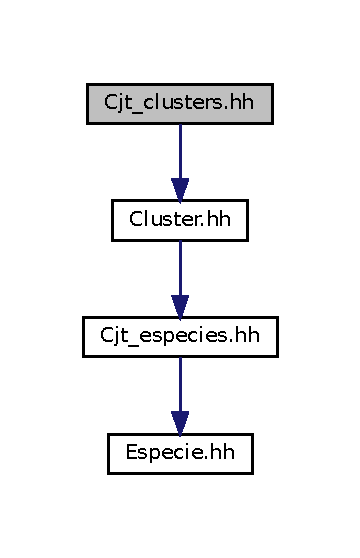
\includegraphics[width=173pt]{_cjt__clusters_8hh__incl}
\end{center}
\end{figure}
\subsection*{Classes}
\begin{DoxyCompactItemize}
\item 
class \hyperlink{class_cjt__clusters}{Cjt\+\_\+clusters}
\begin{DoxyCompactList}\small\item\em Representa un conjunt de clústers. \end{DoxyCompactList}\end{DoxyCompactItemize}


\subsection{Detailed Description}
Especificació de la classe \hyperlink{class_cjt__clusters}{Cjt\+\_\+clusters}. 


\hypertarget{_cjt__especies_8hh}{}\section{Cjt\+\_\+especies.\+hh File Reference}
\label{_cjt__especies_8hh}\index{Cjt\+\_\+especies.\+hh@{Cjt\+\_\+especies.\+hh}}


Especificació de la classe \hyperlink{class_cjt__especies}{Cjt\+\_\+especies}.  


Include dependency graph for Cjt\+\_\+especies.\+hh\+:\nopagebreak
\begin{figure}[H]
\begin{center}
\leavevmode
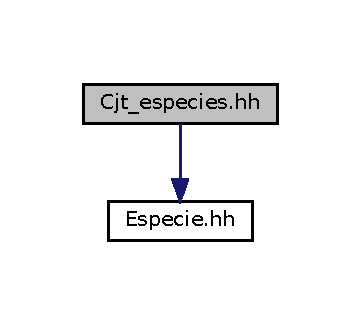
\includegraphics[width=173pt]{_cjt__especies_8hh__incl}
\end{center}
\end{figure}
\subsection*{Classes}
\begin{DoxyCompactItemize}
\item 
class \hyperlink{class_cjt__especies}{Cjt\+\_\+especies}
\begin{DoxyCompactList}\small\item\em Representa un conjunt d\textquotesingle{}espècies. \end{DoxyCompactList}\end{DoxyCompactItemize}


\subsection{Detailed Description}
Especificació de la classe \hyperlink{class_cjt__especies}{Cjt\+\_\+especies}. 


\hypertarget{_cluster_8hh}{}\section{Cluster.\+hh File Reference}
\label{_cluster_8hh}\index{Cluster.\+hh@{Cluster.\+hh}}


Especificació de la classe \hyperlink{class_cluster}{Cluster}.  


Include dependency graph for Cluster.\+hh\+:\nopagebreak
\begin{figure}[H]
\begin{center}
\leavevmode
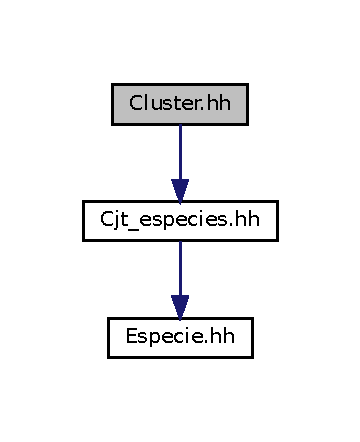
\includegraphics[width=173pt]{_cluster_8hh__incl}
\end{center}
\end{figure}
\subsection*{Classes}
\begin{DoxyCompactItemize}
\item 
class \hyperlink{class_cluster}{Cluster}
\begin{DoxyCompactList}\small\item\em Representa un clúster. \end{DoxyCompactList}\end{DoxyCompactItemize}


\subsection{Detailed Description}
Especificació de la classe \hyperlink{class_cluster}{Cluster}. 


\hypertarget{_especie_8hh}{}\section{Especie.\+hh File Reference}
\label{_especie_8hh}\index{Especie.\+hh@{Especie.\+hh}}


Especificació de la classe \hyperlink{class_especie}{Especie}.  


\subsection*{Classes}
\begin{DoxyCompactItemize}
\item 
class \hyperlink{class_especie}{Especie}
\begin{DoxyCompactList}\small\item\em Representa una entitat o espècie amb atributs identificador i gen. \end{DoxyCompactList}\end{DoxyCompactItemize}


\subsection{Detailed Description}
Especificació de la classe \hyperlink{class_especie}{Especie}. 


\hypertarget{main_8cc}{}\section{main.\+cc File Reference}
\label{main_8cc}\index{main.\+cc@{main.\+cc}}


Programa principal de la {\itshape Construcció d\textquotesingle{}un arbre filogenètic}.  


Include dependency graph for main.\+cc\+:\nopagebreak
\begin{figure}[H]
\begin{center}
\leavevmode
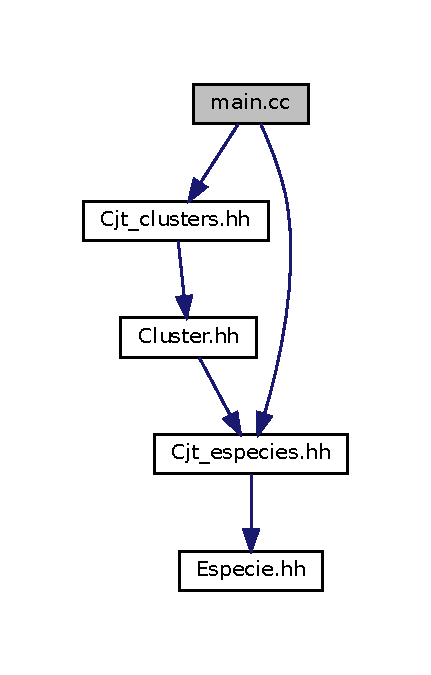
\includegraphics[width=207pt]{main_8cc__incl}
\end{center}
\end{figure}
\subsection*{Functions}
\begin{DoxyCompactItemize}
\item 
int \hyperlink{main_8cc_ae66f6b31b5ad750f1fe042a706a4e3d4}{main} ()
\begin{DoxyCompactList}\small\item\em Programa principal de la {\itshape Construcció d\textquotesingle{}un arbre filogenètic}. \end{DoxyCompactList}\end{DoxyCompactItemize}


\subsection{Detailed Description}
Programa principal de la {\itshape Construcció d\textquotesingle{}un arbre filogenètic}. 



\subsection{Function Documentation}
\mbox{\Hypertarget{main_8cc_ae66f6b31b5ad750f1fe042a706a4e3d4}\label{main_8cc_ae66f6b31b5ad750f1fe042a706a4e3d4}} 
\index{main.\+cc@{main.\+cc}!main@{main}}
\index{main@{main}!main.\+cc@{main.\+cc}}
\subsubsection{\texorpdfstring{main()}{main()}}
{\footnotesize\ttfamily int main (\begin{DoxyParamCaption}{ }\end{DoxyParamCaption})}



Programa principal de la {\itshape Construcció d\textquotesingle{}un arbre filogenètic}. 



Definition at line 22 of file main.\+cc.


\begin{DoxyCode}
22            \{
23     \textcolor{keywordtype}{int} k;
24     cin >> k;
25 
26     \hyperlink{class_cjt__especies}{Cjt\_especies} cesp(k);
27     \hyperlink{class_cjt__clusters}{Cjt\_clusters} cclu;
28 
29     \textcolor{keywordtype}{string} opcio;
30     cin >> opcio;
31 
32     \textcolor{keywordflow}{while} (opcio != \textcolor{stringliteral}{"fin"}) \{
33         \textcolor{keywordflow}{if} (opcio == \textcolor{stringliteral}{"crea\_especie"}) \{
34             \textcolor{keywordtype}{string} id, gen;
35             cin >> \textcolor{keywordtype}{id} >> gen;
36             \hyperlink{class_especie}{Especie} esp (\textcolor{keywordtype}{id}, gen);
37             cesp.crea\_especie(esp);
38         \}
39 
40         \textcolor{keywordflow}{else} \textcolor{keywordflow}{if} (opcio == \textcolor{stringliteral}{"obtener\_gen"}) \{
41             \textcolor{keywordtype}{string} id;
42             cin >> id;
43             cesp.consultar\_especie(\textcolor{keywordtype}{id}).consultar\_gen();
44         \}
45 
46         \textcolor{keywordflow}{else} \textcolor{keywordflow}{if} (opcio == \textcolor{stringliteral}{"distancia"}) \{
47             \textcolor{keywordtype}{string} id1, id2;
48             cin >> id1 >> id2;
49             cesp.distancia(id1, id2);
50         \}
51 
52         \textcolor{keywordflow}{else} \textcolor{keywordflow}{if} (opcio == \textcolor{stringliteral}{"elimina\_especie"}) \{
53             \textcolor{keywordtype}{string} id;
54             cesp.elimina\_especie(\textcolor{keywordtype}{id});
55         \}
56 
57         \textcolor{keywordflow}{else} \textcolor{keywordflow}{if} (opcio == \textcolor{stringliteral}{"existe\_especie"}) \{
58             \textcolor{keywordtype}{string} id;
59             cesp.existeix\_especie(\textcolor{keywordtype}{id});
60         \}
61 
62         \textcolor{keywordflow}{else} \textcolor{keywordflow}{if} (opcio == \textcolor{stringliteral}{"lee\_cjt\_especies"}) \{
63             \textcolor{keywordtype}{int} n;
64             cesp.llegir(n);
65         \}
66 
67         \textcolor{keywordflow}{else} \textcolor{keywordflow}{if} (opcio == \textcolor{stringliteral}{"imprime\_cjt\_especies"}) \{
68             cesp.escriure();
69         \}
70 
71         \textcolor{keywordflow}{else} \textcolor{keywordflow}{if} (opcio == \textcolor{stringliteral}{"tabla\_distancias"}) \{
72             cesp.taula\_distancies();
73         \}
74 
75         \textcolor{keywordflow}{else} \textcolor{keywordflow}{if} (opcio == \textcolor{stringliteral}{"inicializa\_clusters"}) \{
76             cclu.\hyperlink{class_cjt__clusters_a0c0922c708fb014720a53bd560ebed61}{inicialitza\_cluster}(cesp);
77             cclu.\hyperlink{class_cjt__clusters_ab243c775e0e2d64905ce744490d2f898}{taula\_distancies\_clusters}();
78         \}
79 
80         \textcolor{keywordflow}{else} \textcolor{keywordflow}{if} (opcio == \textcolor{stringliteral}{"ejecuta\_paso\_wpgma"}) \{
81             cclu.\hyperlink{class_cjt__clusters_ae5d7fd65b9070ea2e7240d78fefd0f6e}{wpgma\_pas}();
82             cclu.\hyperlink{class_cjt__clusters_ab243c775e0e2d64905ce744490d2f898}{taula\_distancies\_clusters}();
83         \}
84 
85         \textcolor{keywordflow}{else} \textcolor{keywordflow}{if} (opcio == \textcolor{stringliteral}{"imprime\_cluster"}) \{
86             \textcolor{keywordtype}{string} id;
87             cclu.\hyperlink{class_cjt__clusters_ad023ea2a94f2629848f5c6b7162ac8d8}{escriure\_cluster}(\textcolor{keywordtype}{id});
88         \}
89 
90         \textcolor{keywordflow}{else} \textcolor{keywordflow}{if} (opcio == \textcolor{stringliteral}{"imprime\_arbol\_filogenetico"}) \{
91             cclu.\hyperlink{class_cjt__clusters_a0c0922c708fb014720a53bd560ebed61}{inicialitza\_cluster}(cesp);
92             cclu.\hyperlink{class_cjt__clusters_a755fca978c7d4b499e2c7b0963136354}{wpgma\_total}();
93             cclu.\hyperlink{class_cjt__clusters_afdef4a4f7bd8ca2ecaf723c65cc10be0}{escriure\_arbre}();
94         \}
95 
96         cin >> opcio;
97     \}
98 \}
\end{DoxyCode}

%--- End generated contents ---

% Index
\backmatter
\newpage
\phantomsection
\clearemptydoublepage
\addcontentsline{toc}{chapter}{Index}
\printindex

\end{document}
